\documentclass[a4paper,12pt]{report}

% Input encoding and font encoding
\usepackage[utf8]{inputenc}
\usepackage[T1]{fontenc}

\usepackage{multirow}

% Mathematics and symbols
\usepackage{amsmath,amsfonts,amssymb}

% Graphics support and image formats
\usepackage{graphicx}

% Hyperlinks support (hidelinks removes link borders)
\usepackage[hidelinks]{hyperref}

% Enumeration lists customization
\usepackage{enumitem}

% Geometry settings for margins
\usepackage{geometry}
\geometry{margin=1in}

% Table of contents and figures list formatting
\usepackage{tocloft}

% Support for long tables
\usepackage{longtable}

% Acronyms
\usepackage{acronym}

% Language and citation
\usepackage[english]{babel}
\usepackage[superscript]{cite}

% URL formatting in the bibliography
\usepackage{url}

\usepackage{tabularx}
\usepackage{array}
\usepackage[utf8]{inputenc}
\usepackage[table,xcdraw]{xcolor}
\usepackage{caption}
\captionsetup[table]{skip=10pt}
\usepackage{listings}
\lstset{
  backgroundcolor=\color{white},
  basicstyle=\footnotesize\ttfamily,
  breaklines=true,
  frame=single,
  numbers=left,
  numberstyle=\tiny\color{gray},
  stepnumber=1,
  tabsize=2,
  captionpos=b
}
\renewcommand{\lstlistlistingname}{List of Commands}


\begin{document}

% Title page
\begin{titlepage}
    \centering
    \vspace*{1.5cm}
    
    \Huge
    \textbf{Computer Network Project}
    
    \vspace{0.5cm}
    \Large
    Master's in Computer Engineering - Cybersecurity and Systems Administration \\
    Computer Networks (RECOMP)
    
    \vspace{1.5cm}
    
    \vfill

    % Add the logo in the middle of the page
    \includegraphics[width=0.8\textwidth]{figures/isep_wordmark_expanded_vintage.eps}
    
    \vspace{10cm}
    \small
    \textbf{Students} \\
    1250525@isep.ipp.pt | João Araújo \\ 
    1200813@isep.ipp.pt | João Silva  \\
    1200720@isep.ipp.pt | Manuela Leite \\
   
    

    \vspace{0.5cm}
    \small
    \textbf{Responsible professors} \\
    Ana Raquel Faria \\
    Rui Filipe Marques
    
    \vfill
\end{titlepage}

% Table of contents, figures, and acronyms
\pagenumbering{roman}
\tableofcontents
\newpage
\listoffigures
\newpage
\listoftables
\newpage
\lstlistoflistings
\renewcommand{\lstlistingname}{Code}
% Acronyms section
\chapter*{Acronyms}
\begin{acronym}[XXXX] % Use [XXXX] for proper acronym alignment
\acro{WAN}{Wide Area Network}
\acro{HQ}{Headquarters}
\acro{VLAN}{Virtual Local Area Network }
\acro{HSRP}{Hot Standby Router Protocol}
\acro{STP}{Spanning Tree Protocol}
\acro{RSTP}{Rapid Spanning Tree Protocol}
\acro{DHCP}{Dynamic Host Configuration Protocol}
\acro{RECOMP}{Redes de Computadores}
\acro{VTP}{VLAN Trunking Protocol}
\acro{IP}{Internet Protocol}
\acro{SVI}{Switched Virtual Interface}
\end{acronym}

\newpage

\pagenumbering{arabic}

\chapter{Introduction}

This report documents the work completed during Sprint 1 of the \ac{RECOMP} Project, which focuses on the initial configuration and verification of the \ac{RECOMP} Corporation \ac{WAN}. The network spans four geographically distributed sites: Oporto (\ac{HQ}), Warsaw, Munich, and a secure location known as The Vault, all interconnected via the Internet. The initial project state was provided through the packet trace file \texttt{Proj1-start.pkt}.

During Sprint 1, the team carried out the following key activities:

\begin{itemize}
    \item Completed the startup configuration of all routers and switches, ensuring connectivity to the Service Provider network and testing access to external sites such as \texttt{www.google.com}.
    \item Designed and implemented IP addressing schemes for each site based on the allocated address blocks:
    \begin{itemize}
        \item Oporto: 10.21.44.0/22
        \item Warsaw: 192.168.162.0/23
        \item Munich: 172.18.78.0/23
        \item The Vault: 10.31.81.0/24
    \end{itemize}
    \item Configured \ac{VLAN}s, including link aggregation, trunking, and the \ac{VTP} domain across all multilayer and Layer 2 switches.
    \item Implemented \ac{RSTP} and configured \ac{HSRP} for redundancy and high availability.
    \item Configured \ac{DHCP} servers for all \ac{VLAN}s, ensuring that host devices could obtain \ac{IP} addresses automatically.
    \item Verified internal connectivity at each site to confirm that all PCs and network devices were correctly configured.
\end{itemize}

The hardware and network topology at each location were as follows:

\begin{itemize}
    \item \textbf{Oporto (HQ):} 1 × 2911 router, 2 × 3560-24PS multilayer switches, 2 × 2960-24TT Layer 2 switches, and 4 PCs for STAFF, ACCOUNTING, HR, and USERS networks.
    \item \textbf{Warsaw (BR1):} 1 × 2901 router, 3 × 3560-24PS multilayer switches, 4 × 2960-24TT Layer 2 switches, and 4 PCs per VLAN.
    \item \textbf{Munich (BR2):} 2 × 2911 routers, 4 × 2960-24TT Layer 2 switches, and 4 PCs for various networks.
    \item \textbf{The Vault:} 1 × 2911 router and 1 × 2960-24TT Layer 2 switch.
\end{itemize}

The work was distributed among the team as follows:

\begin{itemize}
    \item João Paulo Araujo (1250525@isep.ipp.pt) — Munich \ac{WAN}
    \item João Silva (1200813@isep.ipp.pt) — Warsaw \ac{WAN}
    \item Manuela Leite (1200720@isep.ipp.pt) — Oporto \ac{WAN}
\end{itemize}

This report details the implementation steps, configuration settings, and verification results achieved during Sprint 1, providing the foundation for subsequent sprints in the \ac{RECOMP} Project.

\chapter{Oporto WAN}

\section{Site Overview}

Oporto is the location of the headquarters of the \ac{RECOMP} Corporation and represents the most complex part of the \ac{WAN}. The site consists of the following devices:

\begin{itemize}
    \item One Router HQ (2911 model)
    \item Two Multilayer Switches MLS1 and MLS2 (3560-24PS model)
    \item Two Layer 2 switches (2960-24TT model)
    \item Four PCs representing each of the HQ networks: STAFF, ACCOUNTING, HR and USERS
\end{itemize}

The topology of the Oporto \ac{WAN} is illustrated in Figure~\ref{fig:opo-topology}, showing the connection between the router, multilayer switches, Layer 2 switches, and \ac{VLAN}s for each network.


\begin{figure}[!htb]
\centering
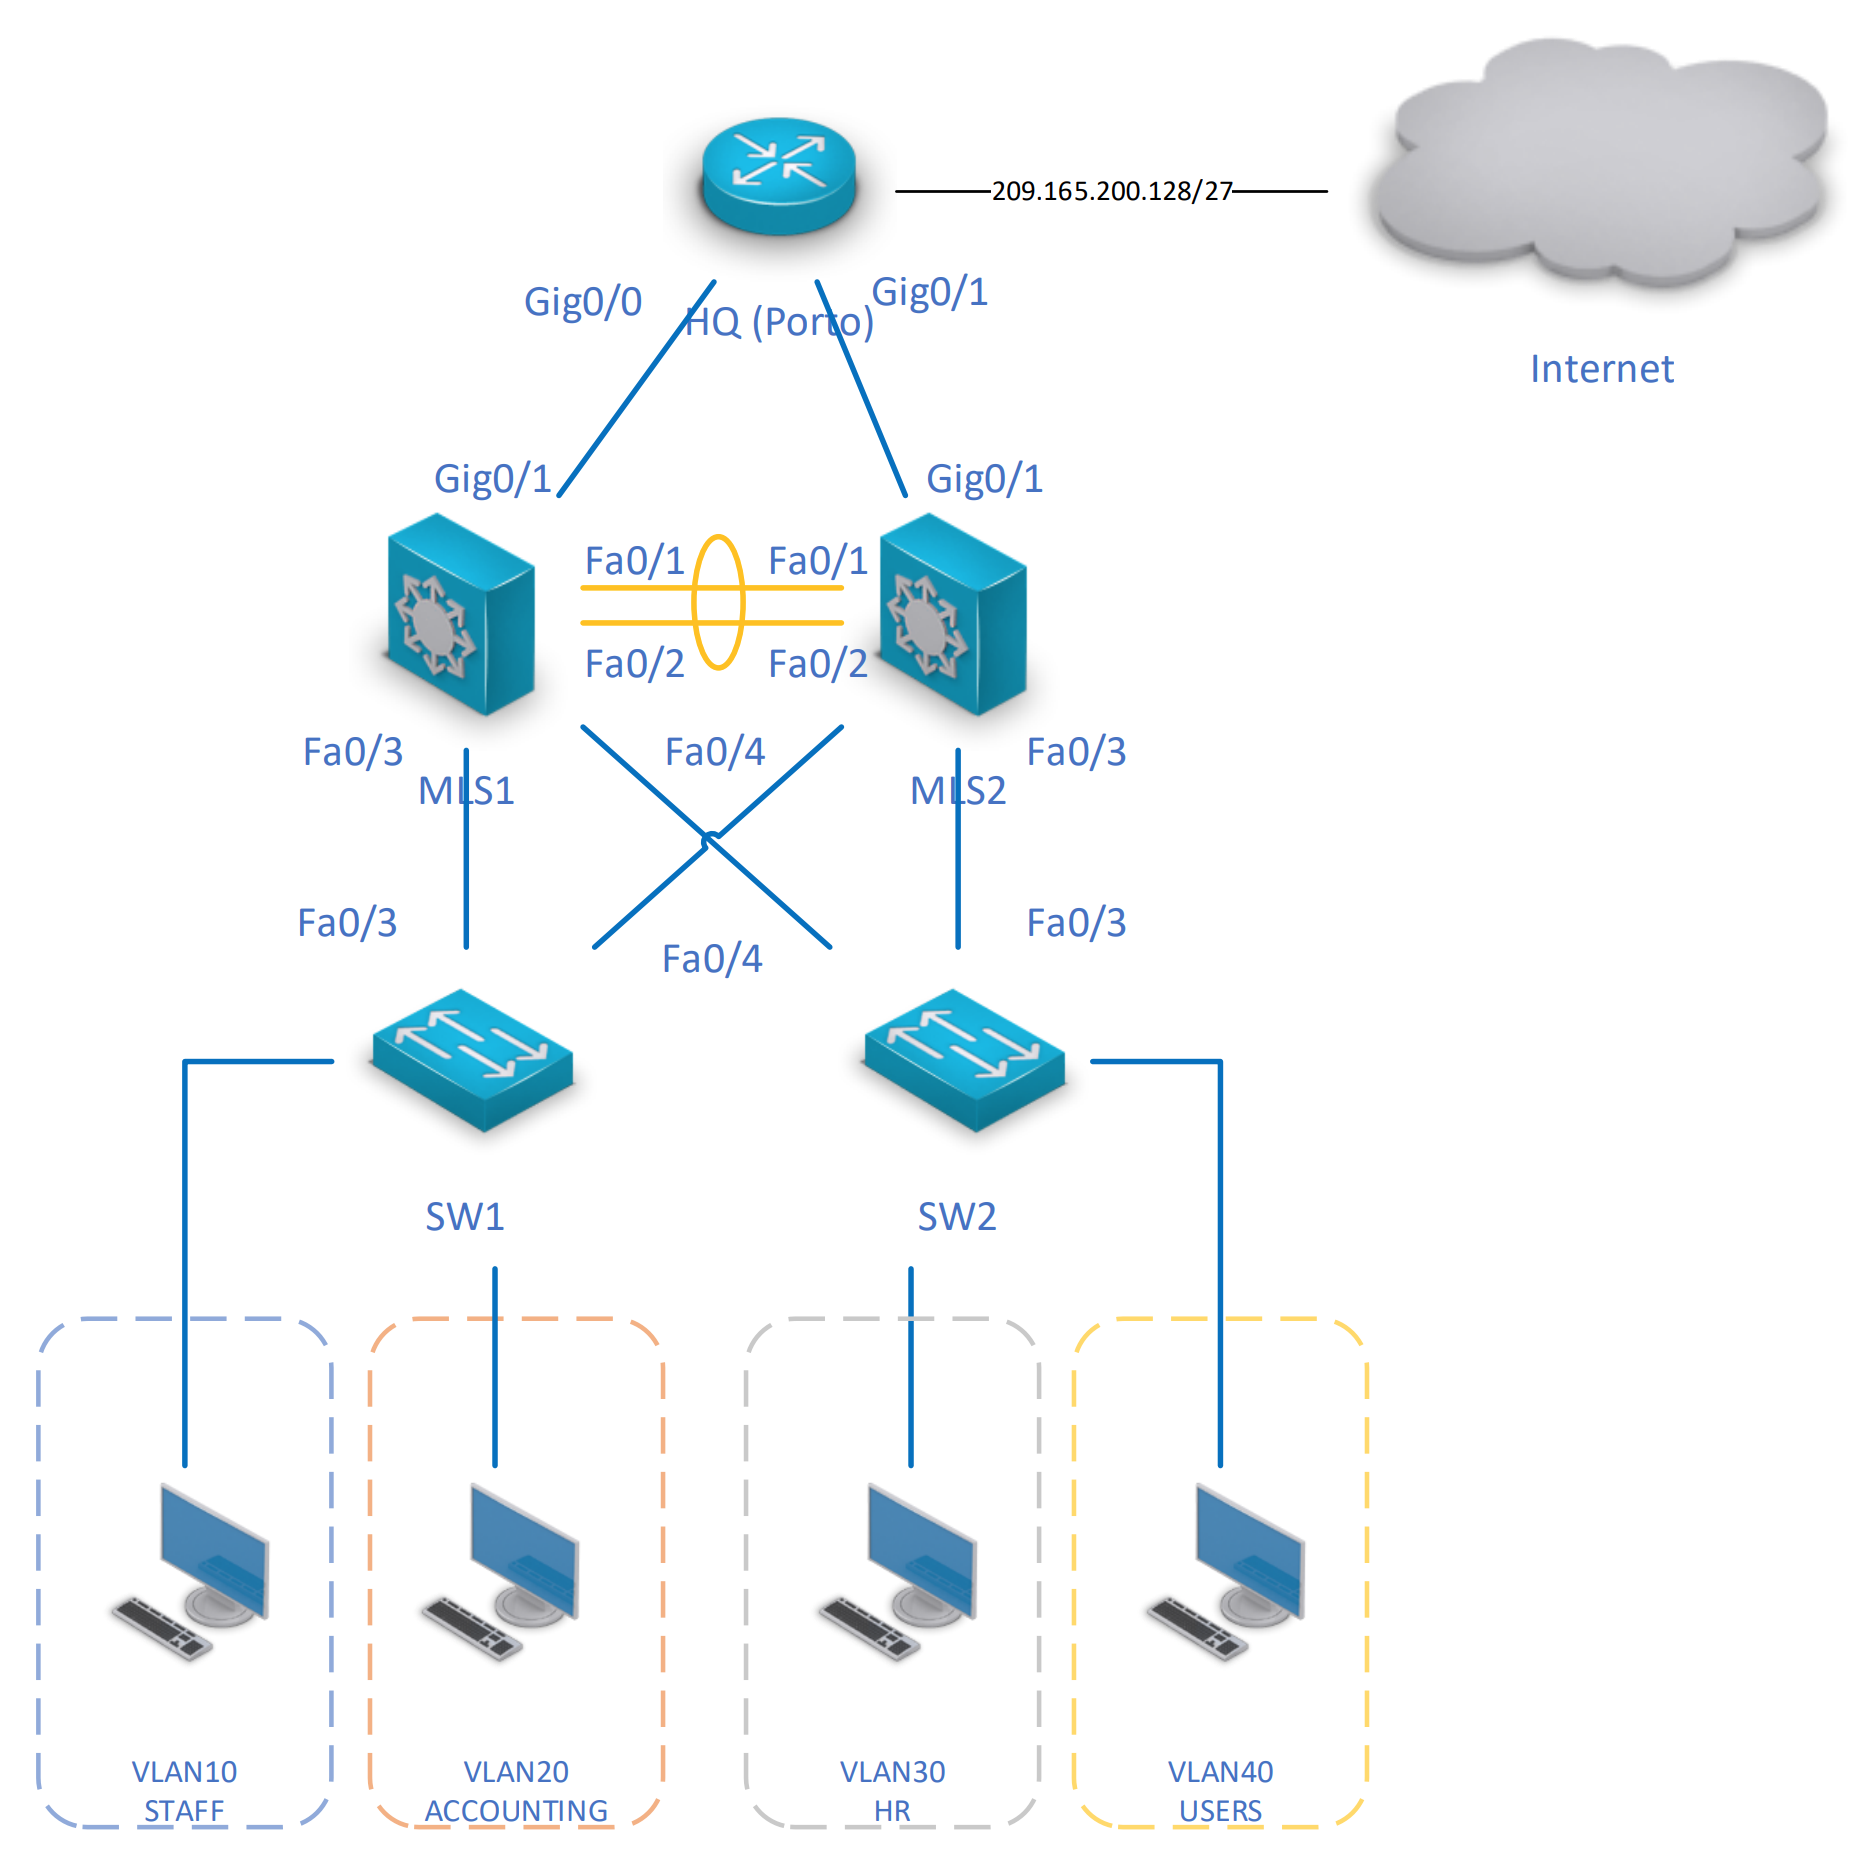
\includegraphics[width=0.5\textwidth]{figures/opo-topology.png}
\caption{Oporto WAN Topology\cite{recomp_sprint1}}
\label{fig:opo-topology}
\end{figure}


The \ac{VLAN}s assigned to the HQ networks are:

\begin{itemize}
    \item \ac{VLAN} 10: STAFF
    \item \ac{VLAN} 20: ACCOUNTING
    \item \ac{VLAN} 30: HR
    \item \ac{VLAN} 40: USERS
\end{itemize}

The Oporto \ac{WAN} is connected to the Internet using the address block 209.165.200.128/27.

\section{Oporto \ac{WAN} Addressing}

The \ac{IP} addressing scheme for the Oporto site was designed to accommodate the four internal networks while optimizing the available address space. The networks and their corresponding addresses are summarized in Table~\ref{tab:opo-addressing}.

\begin{table}[h]
\centering
\resizebox{\textwidth}{!}{%
\begin{tabular}{lccccc}
\hline
Network & Number of Nodes & Network Address & Broadcast Address & Mask & First--Last Valid Address \\
\hline
USERS & 500 & 10.21.44.0 & 10.21.45.255 & /23 & 10.21.44.1 -- 10.21.45.254 \\
ACCOUNTING & 200 & 10.21.46.0 & 10.21.46.255 & /24 & 10.21.46.1 -- 10.21.46.254 \\
HR & 100 & 10.21.47.0 & 10.21.47.127 & /25 & 10.21.47.1 -- 10.21.47.126 \\
STAFF & 50 & 10.21.47.128 & 10.21.47.191 & /26 & 10.21.47.129 -- 10.21.47.190 \\
HQ-ROUTER $\leftrightarrow$ MLS1 & 4 & 10.21.47.192 & 10.21.47.195 & /30 & 10.21.47.193-10.21.47.194 \\
HQ-ROUTER $\leftrightarrow$ MLS2 & 4 & 10.21.47.196 & 10.21.47.199 & /30 & 10.21.47.197-10.21.47.198 \\
\hline
\end{tabular}%
}
\caption{Oporto \ac{WAN} \ac{IP} addressing scheme.}
\label{tab:opo-addressing}
\end{table}


\begin{figure}[!htb]
\centering
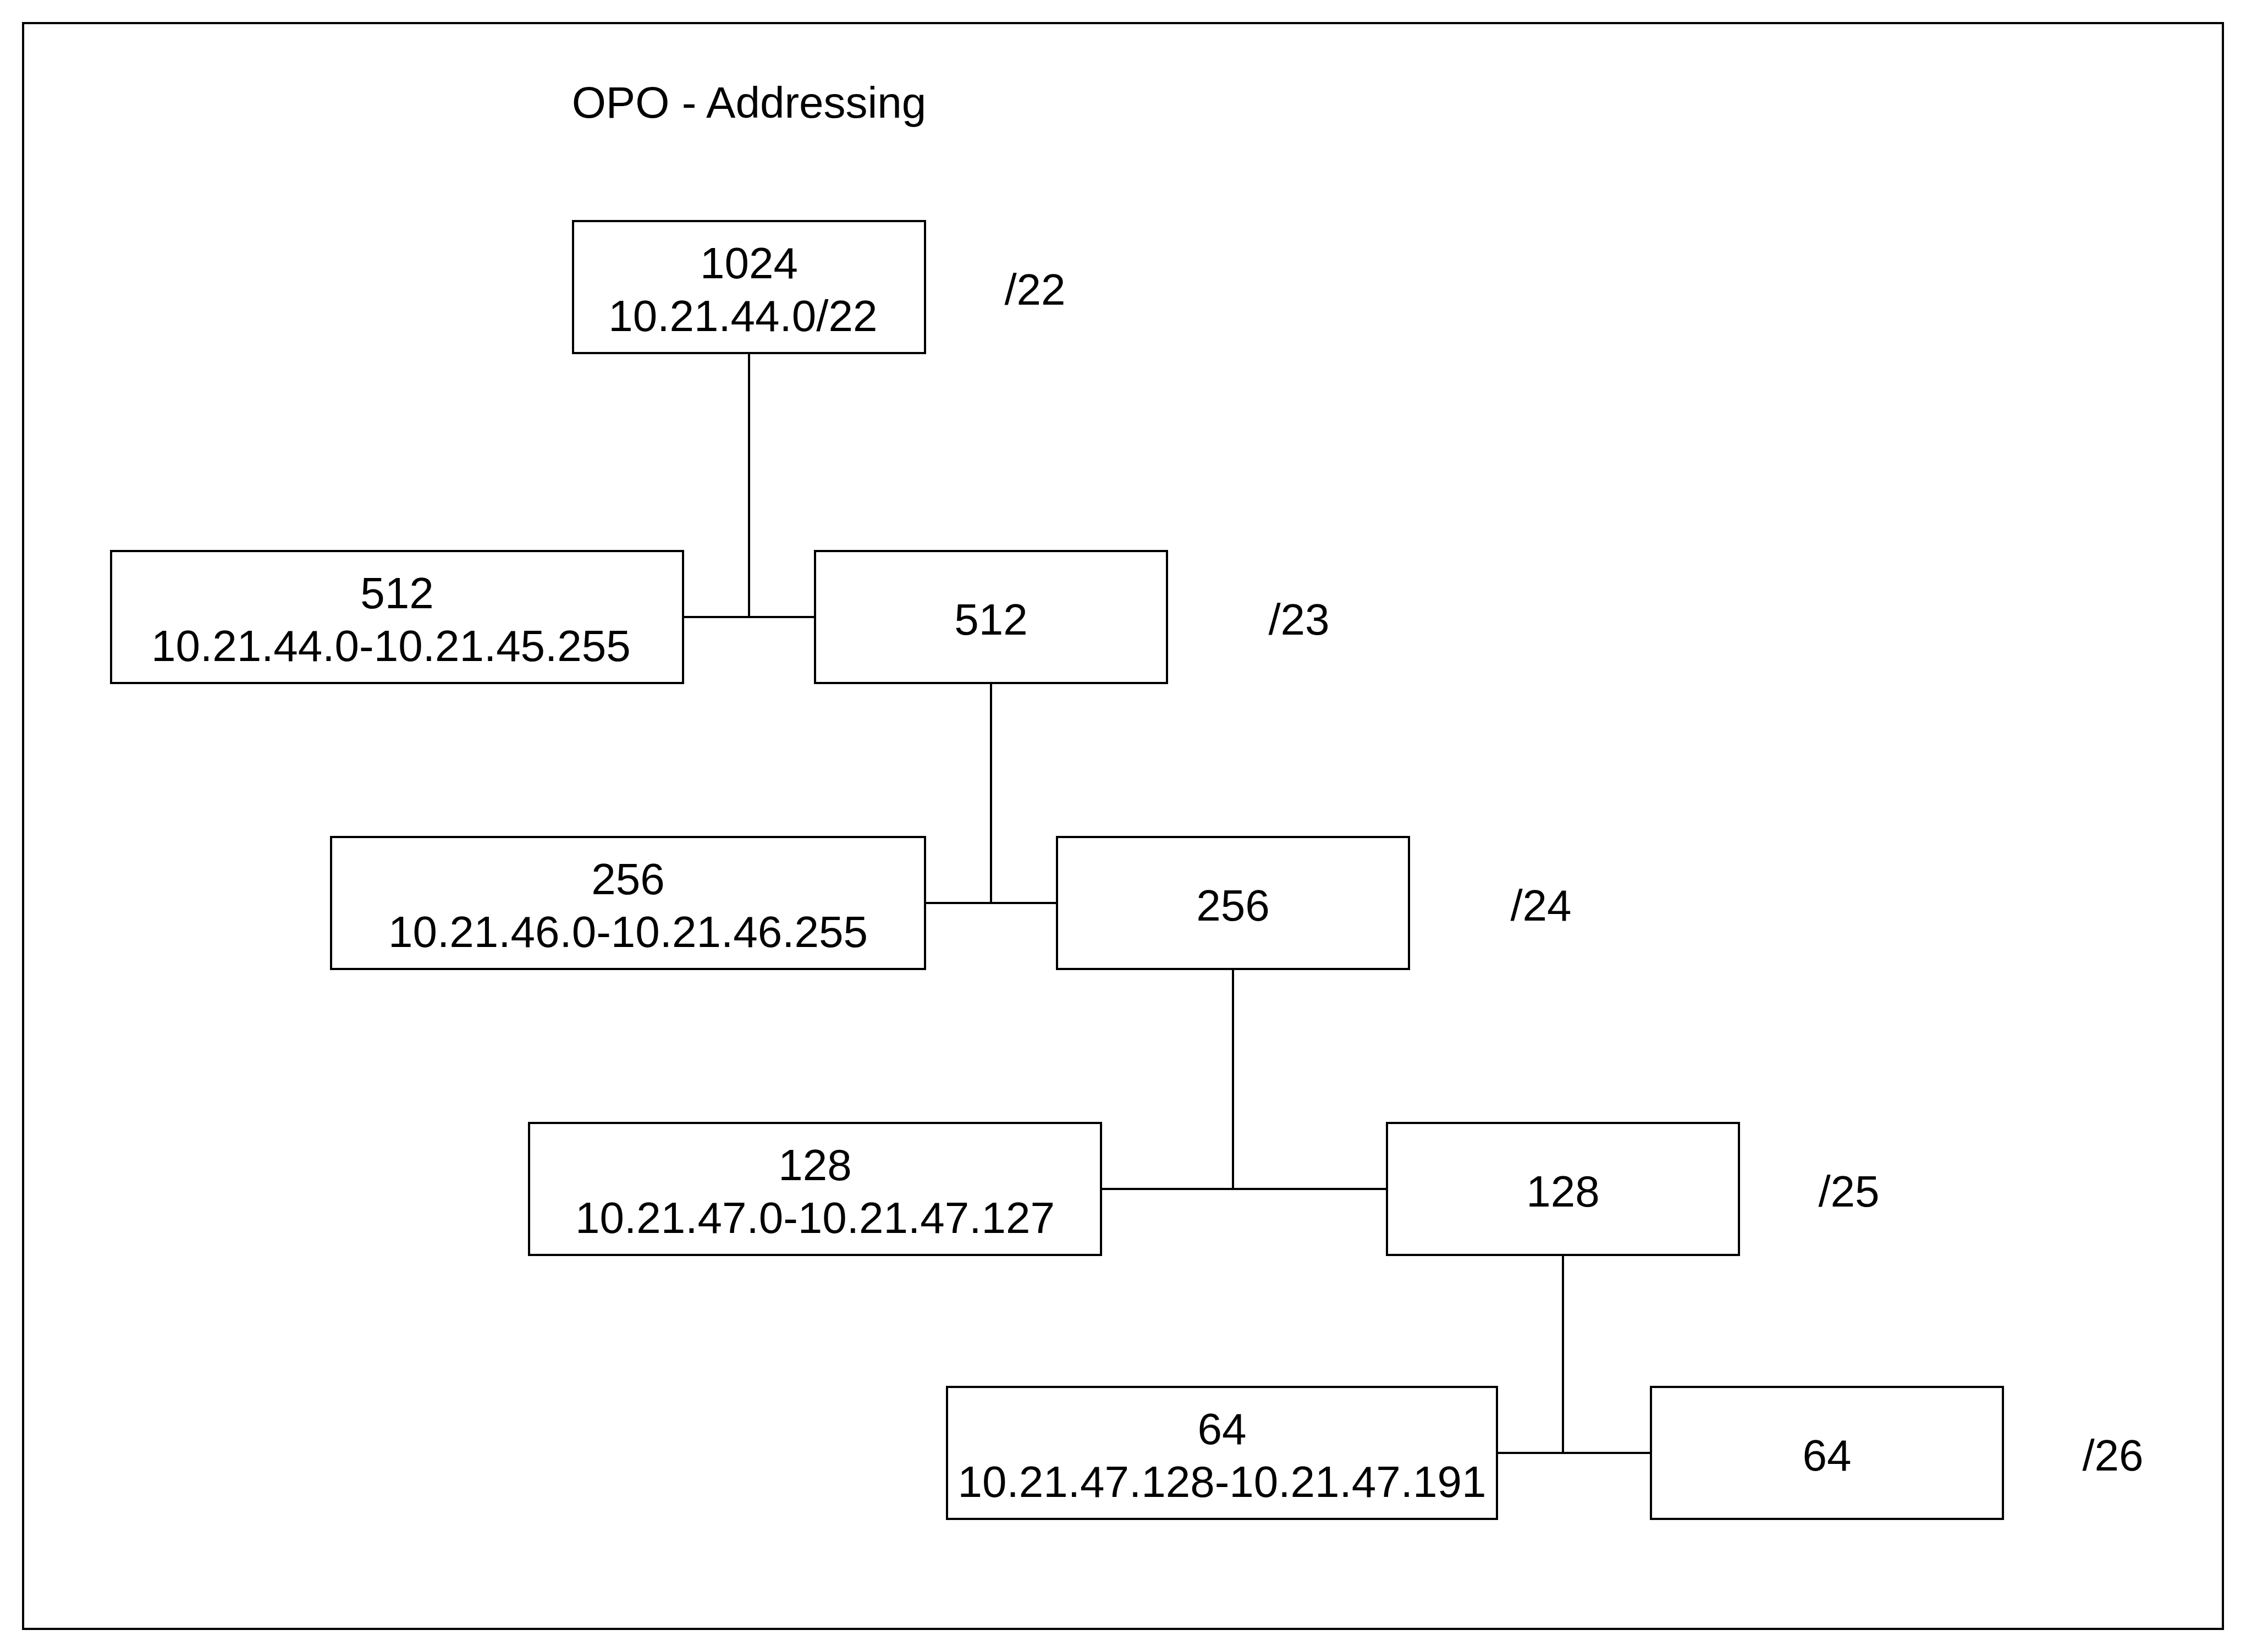
\includegraphics[width=0.8\textwidth]{figures/opo-addressing.png}
\caption{Oporto \ac{WAN} Addressing Diagram\cite{t3a_ipv4_subneting_dhcp}}
\label{fig:opo-addressing}
\end{figure}

This addressing plan ensures that each network has sufficient \ac{IP} addresses to accommodate all devices, while also allowing room for potential future expansion. The subnet sizes were calculated based on the number of hosts in each network, following standard subnetting rules.

\subsection{Equipment Addressing}

The \ac{IP} addresses listed in Table~\ref{tab:ip-plan} correspond to statically assigned management and gateway interfaces within the Oporto headquarters network. These addresses are \textbf{excluded from \ac{DHCP}} to prevent dynamic clients from receiving them.

\medskip

Each VLAN has three reserved addresses:
\begin{itemize}
    \item The \textbf{\ac{HSRP} virtual gateway}, used by hosts as their default gateway.
    \item The \textbf{\ac{SVI} address on MLS1}.
    \item The \textbf{\ac{SVI} address on MLS2}.
\end{itemize}

\noindent
These static \ac{IP}s ensure stable Layer~3 routing and redundancy between MLS1 and MLS2. All other addresses within the \ac{VLAN} subnet ranges are assigned dynamically by the \ac{DHCP} server.


\begin{table}[h!]
\centering
\caption{Network Equipment and Assigned IP Addresses Oporto WAN}
\resizebox{\textwidth}{!}{%
\begin{tabular}{l l l l}
\hline
\textbf{Device} & \textbf{Interface / VLAN} & \textbf{IP Address} & \textbf{Description / Function} \\
\hline
\textbf{HQ Router (2911)} & G0/0 & 10.21.47.193 /30 & Link to MLS1 \\
                          & G0/1 & 10.21.47.197 /30 & Link to MLS2 \\
                          & G0/0/0 & DHCP (Public) & WAN connection to ISP \\[4pt]
\textbf{MLS1 (3560-24PS)} & VLAN10 & 10.21.47.130 /26 & STAFF SVI (HSRP Active) \\
                          & VLAN20 & 10.21.46.2 /24 & ACCOUNTING SVI (HSRP Active) \\
                          & VLAN30 & 10.21.47.2 /25 & HR SVI (HSRP Standby) \\
                          & VLAN40 & 10.21.44.2 /23 & USERS SVI (HSRP Standby) \\
                          & G0/1 & 10.21.47.194 /30 & Link to HQ Router \\[4pt]
\textbf{MLS2 (3560-24PS)} & VLAN10 & 10.21.47.131 /26 & STAFF SVI (HSRP Standby) \\
                          & VLAN20 & 10.21.46.3 /24 & ACCOUNTING SVI (HSRP Standby) \\
                          & VLAN30 & 10.21.47.3 /25 & HR SVI (HSRP Active) \\
                          & VLAN40 & 10.21.44.3 /23 & USERS SVI (HSRP Active) \\
                          & G0/1 & 10.21.47.198 /30 & Link to HQ Router \\[4pt]
\textbf{HSRP Virtual IPs} & VLAN10 & 10.21.47.129 /26 & STAFF Gateway (Virtual) \\
                          & VLAN20 & 10.21.46.1 /24 & ACCOUNTING Gateway (Virtual) \\
                          & VLAN30 & 10.21.47.1 /25 & HR Gateway (Virtual) \\
                          & VLAN40 & 10.21.44.1 /23 & USERS Gateway (Virtual) \\[4pt]
\textbf{SW1, SW2 (2960-24TT)} & Trunk links & N/A & Access layer switches, VTP clients \\[4pt]
\textbf{End Device (PC1)} & VLAN10 & DHCP assigned & STAFF network client \\
\textbf{End Device (PC2)} & VLAN20 & DHCP assigned & ACCOUNTING network client \\
\textbf{End Device (PC3)} & VLAN30 & DHCP assigned & HR network client \\
\textbf{End Device (PC4)} & VLAN40 & DHCP assigned & USERS network client \\
\hline
\end{tabular}%
}
\label{tab:ip-plan}
\end{table}

\section{Configuration}

\subsection{HQ Router and MLS Configuration}
The HQ Router obtains its external \ac{IP} address from the Service Provider via \ac{DHCP}, while the internal connections between the HQ Router and the multilayer switches (MLS1 and MLS2) are configured with static \ac{IP} addresses.  
This ensures consistent routing and stable communication between the HQ and internal networks.

\begin{lstlisting}[caption={HQ Router configuration}, label={lst:hq-router}]
enable
configure terminal

! Internal connection to MLS1
interface GigabitEthernet0/0
 description HQ-MLS1 Connection
 ip address 10.21.47.193 255.255.255.252
 no shutdown
exit

! Internal connection to MLS2
interface GigabitEthernet0/1
 description HQ-MLS2 Connection
 ip address 10.21.47.197 255.255.255.252
 no shutdown
exit

! External connection to Service Provider (WAN)
interface GigabitEthernet0/0/0
 description Service Provider Connection
 ip address dhcp
 no shutdown
exit

! Default route to the Internet (through SP)
ip route 0.0.0.0 0.0.0.0 GigabitEthernet0/0/0
end
\end{lstlisting}

The static \ac{IP}s configured on the HQ Router correspond to the point-to-point subnets used for internal routing with MLS1 and MLS2.

\begin{lstlisting}[caption={MLS1 link to HQ Router}, label={lst:mls1-router-link}]
enable
configure terminal
interface GigabitEthernet0/1
 description Link to HQ Router
 no switchport
 ip address 10.21.47.194 255.255.255.252
 no shutdown
end
\end{lstlisting}

\begin{lstlisting}[caption={MLS2 link to HQ Router}, label={lst:mls2-router-link}]
enable
configure terminal
interface GigabitEthernet0/1
 description Link to HQ Router
 no switchport
 ip address 10.21.47.198 255.255.255.252
 no shutdown
end
\end{lstlisting}

This configuration guarantees reliable Layer~3 communication between the HQ Router and both MLS devices.  
By assigning static \ac{IP} addresses internally and using \ac{DHCP} externally, the HQ Router maintains dynamic Internet access while ensuring stable connectivity with the local switching infrastructure.


\begin{lstlisting}[caption={Access port configuration on SW1 and SW2}, label={lst:sw1-sw2-access}]
interface range fa0/5 - 8
 switchport mode access
 switchport access vlan 10
!
interface range fa0/9 - 12
 switchport mode access
 switchport access vlan 20
!
interface range fa0/13 - 16
 switchport mode access
 switchport access vlan 30
!
interface range fa0/17 - 20
 switchport mode access
 switchport access vlan 40
!
interface range fa0/1 - 4, fa0/21 - 24
 switchport access vlan 99
 shutdown
\end{lstlisting}

\subsection{\ac{VTP} and \ac{VLAN} Configuration}

\ac{VTP} was implemented on the HQ switches in order to automate \ac{VLAN} propagation.  
MLS1 and MLS2 were configured as \ac{VTP} servers and SW1 and SW2 as clients.  
This ensures that \ac{VLAN} information is consistent across all switches.

\begin{lstlisting}[caption={VTP configuration on MLS1 and MLS2}, label={lst:vtp-config}]
vtp domain RECOMP2526TTTGG
vtp password 6252pmocer
vtp mode server
\end{lstlisting}

\begin{lstlisting}[caption={VTP configuration on SW1 and SW2}, label={lst:vtp-clients}]
vtp domain RECOMP2526TTTGG
vtp password 6252pmocer
vtp mode client
\end{lstlisting}

\ac{VLAN}s were created on the MLS switches to segment traffic per department, improving security and broadcast efficiency.

\begin{lstlisting}[caption={VLAN creation on MLS1 and MLS2\cite{tp2_layer2_security}}, label={lst:mls1-msl2-vlans}]
vlan 10 name STAFF
vlan 20 name ACCOUNTING
vlan 30 name HR
vlan 40 name USERS
vlan 50 name NATIVE
vlan 99 name BLACKHOLE
\end{lstlisting}

\subsection{Trunk and Port-Channel Configuration}
To provide redundancy and increased bandwidth between MLS1 and MLS2, a Port-Channel was configured using interfaces \texttt{Fa0/1–2}.  
All inter-switch links were configured as trunks, using \ac{VLAN}~50 as the native \ac{VLAN}.

\begin{lstlisting}[caption={Trunk and Port-Channel configuration on MLS1 and MLS2}, label={lst:mls1-portchannel}]
interface range fa0/1 - 2
 channel-group 1 mode active
!
interface port-channel 1
 switchport trunk encapsulation dot1q
 switchport mode trunk
 switchport trunk allowed vlan all
 switchport trunk native vlan 50
!
interface range fa0/3 - 4
 switchport mode trunk
 switchport trunk allowed vlan all
 switchport trunk native vlan 50
 no shutdown
\end{lstlisting}

This design allows all \ac{VLAN}s to traverse the trunks, ensuring communication between switches and minimizing single points of failure.

\subsection{\ac{RSTP}}
Rapid-PVST was used to optimize convergence and redundancy.  
Root bridge roles were manually assigned to balance \ac{VLAN} traffic: MLS1 for \ac{VLAN}s 10 and 20, and MLS2 for \ac{VLAN}s 30 and 40.

\begin{lstlisting}[caption={RSTP configuration on MLS1}, label={lst:rstp-mls1}]
spanning-tree mode rapid-pvst
spanning-tree vlan 10,20 root primary
spanning-tree vlan 30,40 root secondary
\end{lstlisting}

\begin{lstlisting}[caption={RSTP configuration on MLS2}, label={lst:rstp-mls2}]
spanning-tree mode rapid-pvst
spanning-tree vlan 30,40 root primary
spanning-tree vlan 10,20 root secondary
\end{lstlisting}

This configuration ensures load balancing and prevents loops, as each switch becomes the primary root for specific \ac{VLAN}s.

\subsection{\ac{HSRP} Configuration}
\ac{HSRP} was configured on both MLS switches to provide default gateway redundancy.  
Each \ac{VLAN} has a virtual gateway IP, and the active MLS for each \ac{VLAN} matches its \ac{STP} root, optimizing path efficiency.

\begin{lstlisting}[caption={HSRP configuration on MLS1}, label={lst:hsrp-mls1}]
ip routing
!
interface vlan10
 ip address 10.21.47.130 255.255.255.192
 standby 10 ip 10.21.47.129
 standby 10 priority 110
 standby 10 preempt
!
interface vlan20
 ip address 10.21.46.2 255.255.255.0
 standby 20 ip 10.21.46.1
 standby 20 priority 110
 standby 20 preempt
\end{lstlisting}

\begin{lstlisting}[caption={HSRP configuration on MLS2}, label={lst:hsrp-mls2}]
ip routing
!
interface vlan30
 ip address 10.21.47.3 255.255.255.128
 standby 30 ip 10.21.47.1
 standby 30 priority 110
 standby 30 preempt
!
interface vlan40
 ip address 10.21.44.3 255.255.254.0
 standby 40 ip 10.21.44.1
 standby 40 priority 110
 standby 40 preempt
\end{lstlisting}

This setup guarantees seamless failover for gateway services in the event one switch fails.

\subsection{Layer 2 Switch Configuration}
SW1 and SW2 were configured to connect end devices to the correct \ac{VLAN}s and isolate unused ports.

\begin{lstlisting}[caption={Access port configuration on SW1 and SW2}, label={lst:sw1-access}]
interface range fa0/5 - 8
 switchport mode access
 switchport access vlan 10
!
interface range fa0/9 - 12
 switchport mode access
 switchport access vlan 20
!
interface range fa0/13 - 16
 switchport mode access
 switchport access vlan 30
!
interface range fa0/17 - 20
 switchport mode access
 switchport access vlan 40
!
interface range fa0/1 - 4, fa0/21 - 24
 switchport access vlan 99
 shutdown
\end{lstlisting}

Unused ports were placed in VLAN~99 and shut down to enhance security and prevent unauthorized connections.

\subsection{DHCP Configuration}
Redundant \ac{DHCP} services were configured on both MLS switches.  
Each \ac{VLAN} has its own pool, while addresses used by \ac{HSRP} and \ac{SVI}s were excluded to avoid conflicts.

\begin{lstlisting}[caption={DHCP configuration on MLS1 and MLS2}, label={lst:dhcp-mls}]
ip dhcp excluded-address 10.21.47.129 10.21.47.131
ip dhcp excluded-address 10.21.46.1 10.21.46.3
ip dhcp excluded-address 10.21.47.1 10.21.47.3
ip dhcp excluded-address 10.21.44.1 10.21.44.3
!
ip dhcp pool STAFF
 network 10.21.47.128 255.255.255.192
 default-router 10.21.47.129
 dns-server 8.8.8.8
 domain-name recomp2526.com
\end{lstlisting}

This ensures reliable address distribution and gateway redundancy across all \ac{VLAN}s.



\chapter{Warsaw WAN}

\section{Site Overview}
The Warsaw site is one of the three main locations in the \ac{RECOMP} Corporation architecture. His structure includes the following key components:
\begin{itemize}
    \item Tree core multilayer switches (3560-24PS model).
    \item One router (2901 model).
    \item Four layer 2 switches (2960-24TT model).
    \item  Four PCs representing each of the networks (STAFF, ACCOUNTING, HR, USERS).
    \end{itemize}


The topology of the warsaw site is illustrated in Figure~\ref{fig:warsaw-topology}, showcasing the interconnections between the core switches, router, layer 2 switches, and PCs.

\begin{figure}[h!]
    \centering
    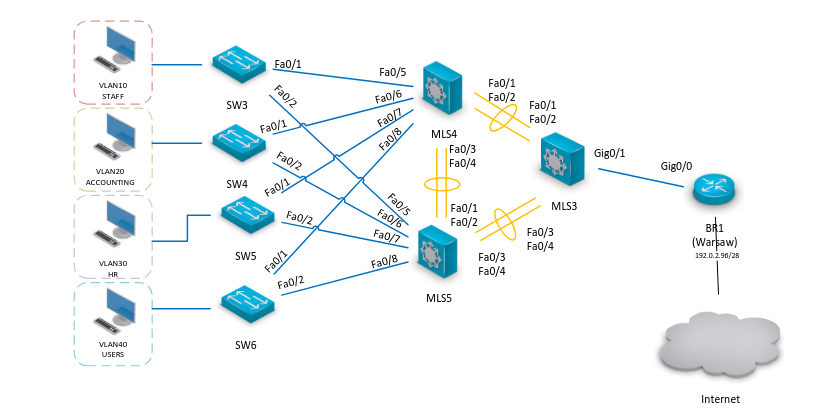
\includegraphics[width=0.9\textwidth]{figures/warsaw-topology.png}
    \caption{Warsaw Site Topology}
    \label{fig:warsaw-topology}
\end{figure}



\section{IP Addressing Scheme}
The Warsaw network architecture is built upon a structured IP plan. The following tables detail the VLAN subnets and the specific IP addresses assigned to core network devices.

\section{VLAN Subnet Allocation}

\begin{table}[h!]
\centering
\caption{VLAN Subnet Allocation}
\resizebox{\textwidth}{!}{%
\begin{tabular}{|l|c|c|c|c|c|}
\hline
\textbf{VLAN Name} & \textbf{VLAN ID} & \textbf{Network ID} & \textbf{Mask} & \textbf{Usable IP Range} & \textbf{Broadcast} \\
\hline
USERS & 40 & 192.168.162.0 & /24 & 192.168.162.1 -- 192.168.162.254 & 192.168.162.255 \\
\hline
STAFF & 10 & 192.168.163.0 & /27 & 192.168.163.1 -- 192.168.163.30 & 192.168.163.31 \\
\hline
ACCOUNTING & 20 & 192.168.163.32 & /27 & 192.168.163.33 -- 192.168.163.62 & 192.168.163.63 \\
\hline
HR & 30 & 192.168.163.64 & /27 & 192.168.163.65 -- 192.168.163.94 & 192.168.163.95 \\
\hline
\end{tabular}%
}
\label{tab:warsaw-vlan}
\end{table}

As the figure \ref{fig:warsaw-addressing} shows, the VLANs were designed to accommodate the minimum number of hosts required, also with additional capacity for future growth.

\begin{figure}[h!]
    \centering
    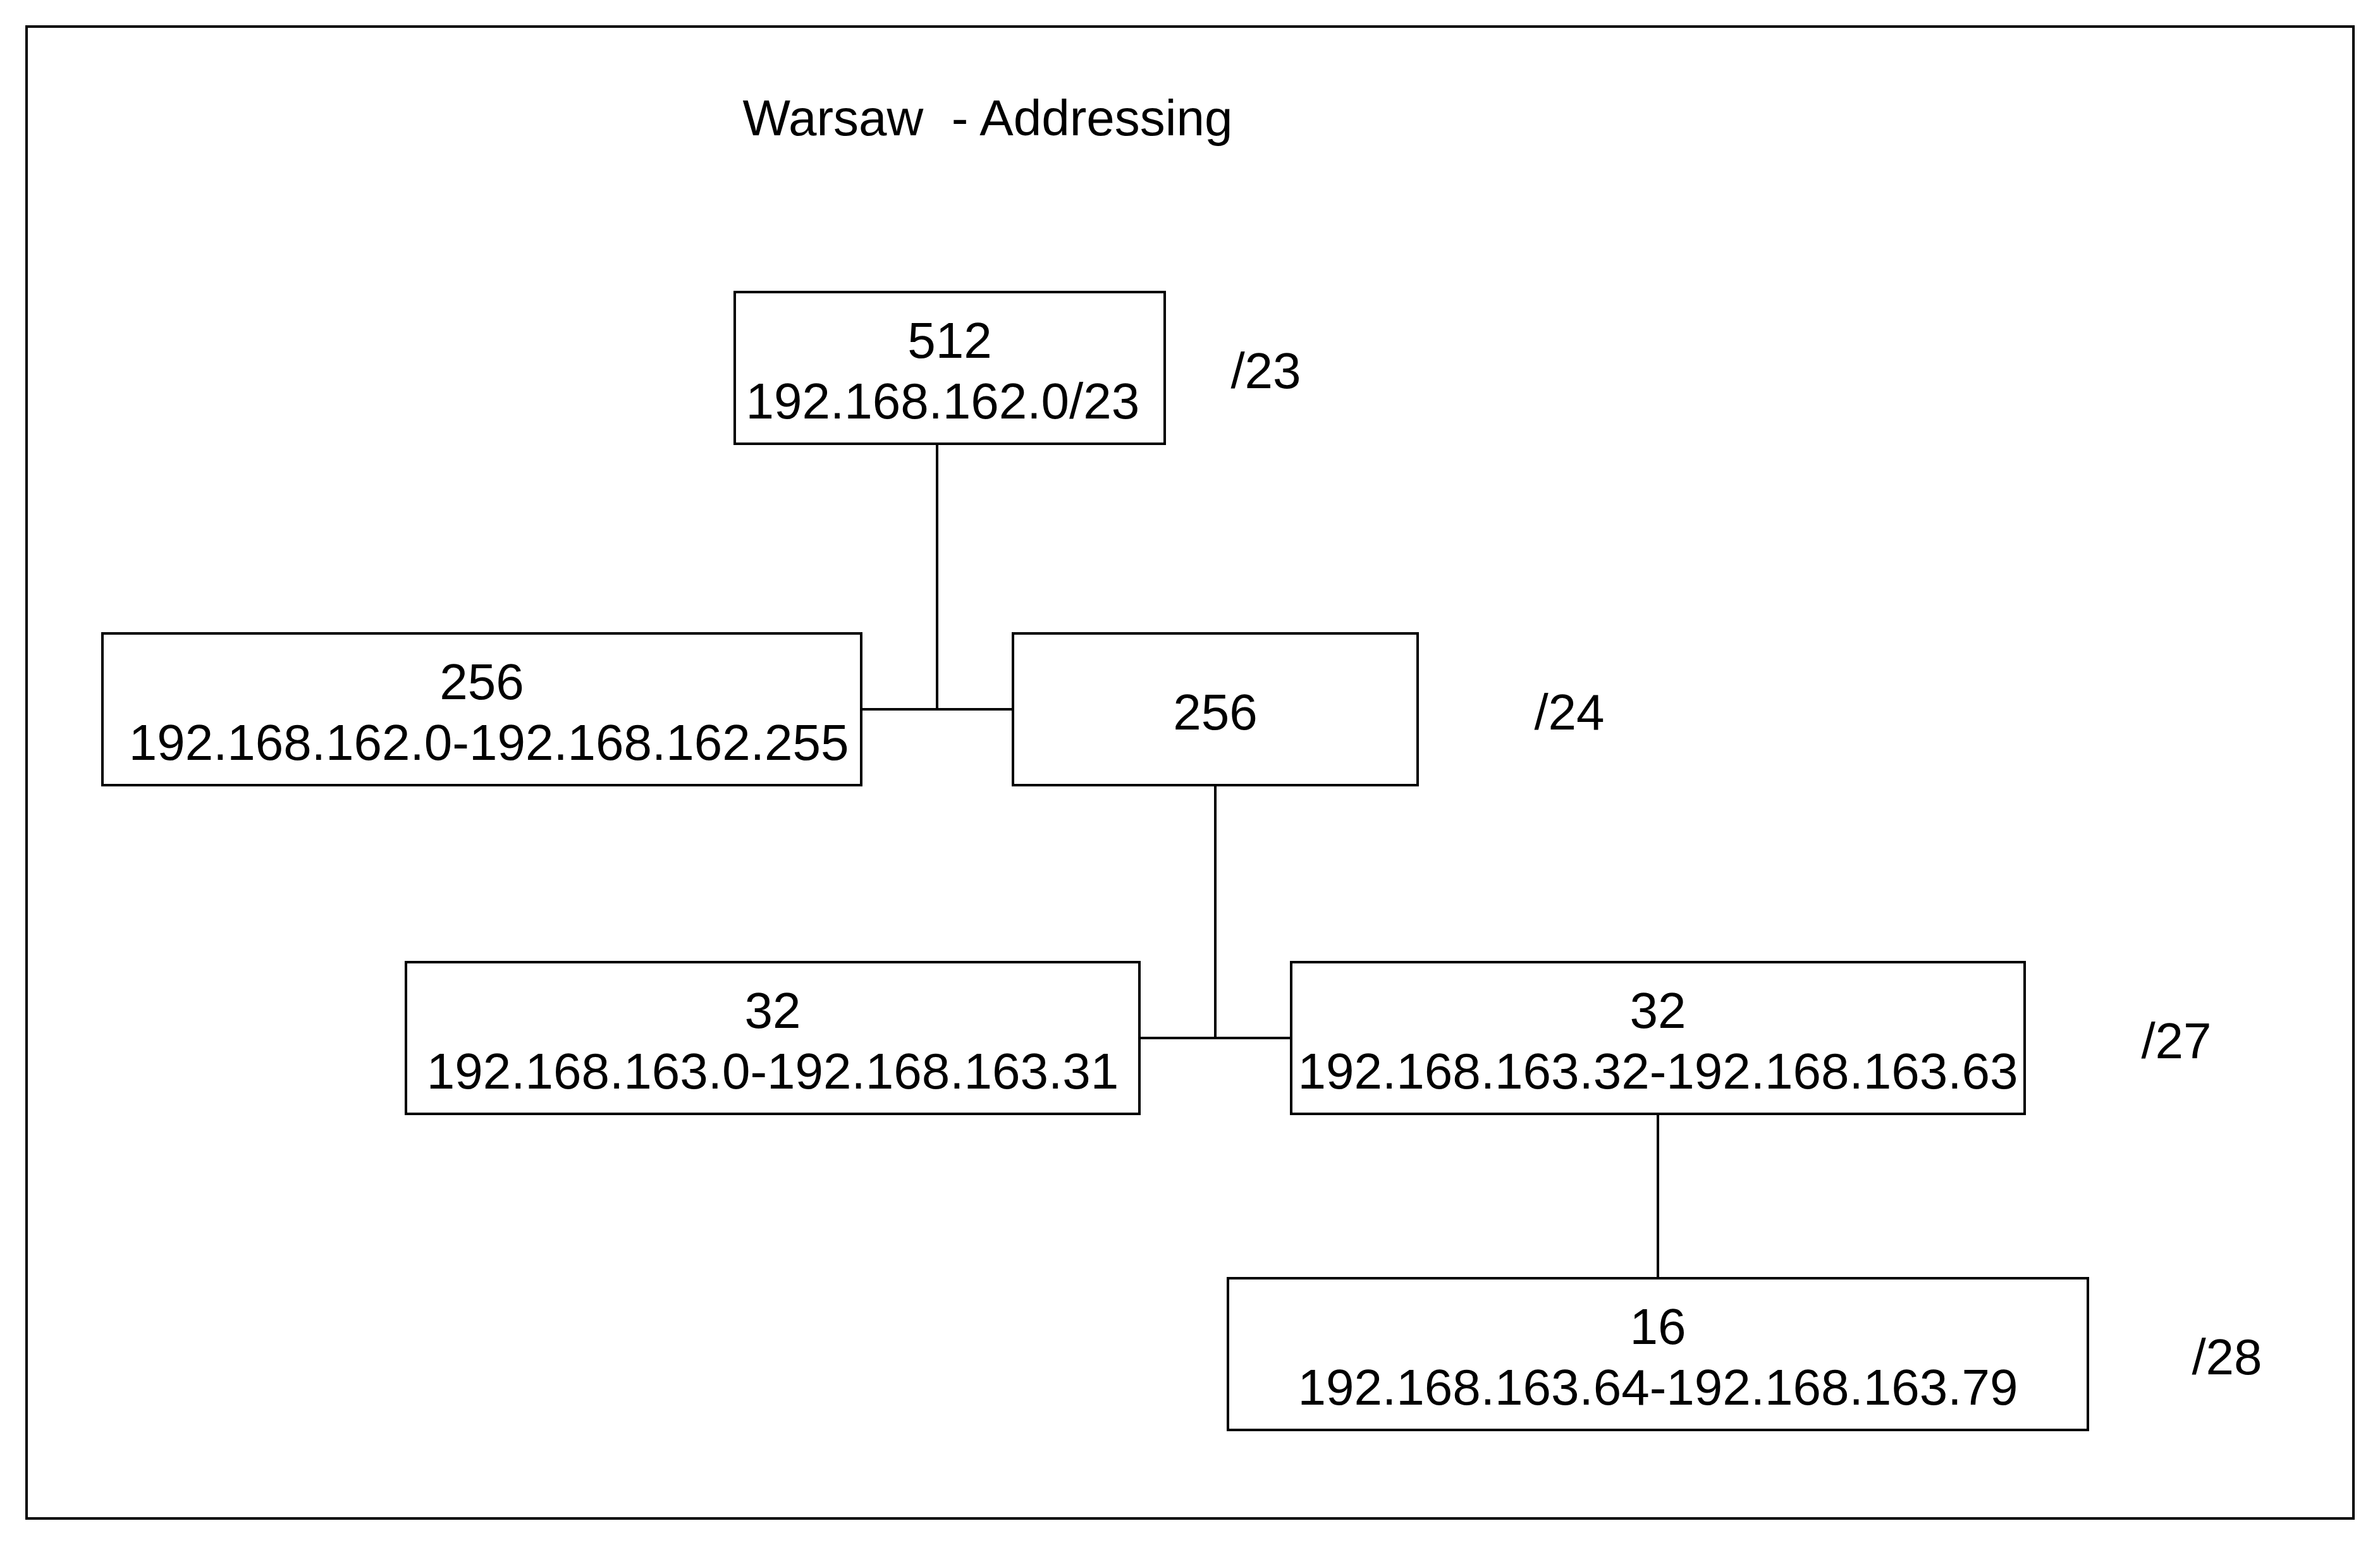
\includegraphics[width=0.9\textwidth]{figures/warsaw-addressing.png}
    \caption{Warsaw IP Addressing Scheme}
    \label{fig:warsaw-addressing}
\end{figure}    

\section{Core Device Interface Assignments}

Static IP addresses were assigned to core multilayer switch (MLS) interfaces for routing.
\begin{table}[h!]
\centering
\caption{Core Device Interface Assignments}
\begin{tabular}{|l|l|c|}
\hline
\textbf{Device} & \textbf{Interface} & \textbf{IP Address / Mask} \\

\hline
\multirow{5}{*}{MLS4} 
                      & VLAN 10 & 192.168.163.2 /27 \\
                      & VLAN 20 & 192.168.163.34 /27 \\
                      & VLAN 30 & 192.168.163.66 /27 \\
                      & VLAN 40 & 192.168.162.2 /24 \\
\hline
\multirow{5}{*}{MLS5} 
                      & VLAN 10 & 192.168.163.3 /27 \\
                      & VLAN 20 & 192.168.163.35 /27 \\
                      & VLAN 30 & 192.168.163.67 /27 \\
                      & VLAN 40 & 192.168.162.3 /24 \\
\hline
\end{tabular}
\label{tab:warsaw-core}
\end{table}


\section{Core Device Configuration}

The following command sets were applied to the core multilayer switches to establish VLANs, routing, and redundancy.

\subsection{VLAN and VTP Configuration}

VLAN Trunking Protocol (VTP) was configured to synchronize VLAN databases across the Warsaw switching domain.  
All multilayer switches operate in \texttt{server} mode to ensure database consistency and integrity.

\begin{lstlisting}[caption={VLAN and VTP configuration}, label={lst:warsaw-vtp}]
vtp mode server
vtp domain RECOMP2526M1A06
vtp password 6252pmocer

vlan 10
 name STAFF
vlan 20
 name ACCOUNTING
vlan 30
 name HR
vlan 40
 name USERS
vlan 50
 name NATIVE
vlan 99
 name BLACKHOLE
ip routing
\end{lstlisting}

\subsection{Spanning Tree Protocol \ac{STP} Configuration}

Rapid Per-VLAN Spanning Tree (Rapid-PVST) was enabled to maintain a loop-free topology and to provide load balancing between core switches.

\begin{lstlisting}[caption={RSTP configuration on MLS4}, label={lst:warsaw-rstp-mls4}]
spanning-tree mode rapid-pvst
spanning-tree vlan 10,20 root primary
spanning-tree vlan 30,40 root secondary
\end{lstlisting}

\begin{lstlisting}[caption={RSTP configuration on MLS5}, label={lst:warsaw-rstp-mls5}]
spanning-tree mode rapid-pvst
spanning-tree vlan 30,40 root primary
spanning-tree vlan 10,20 root secondary
\end{lstlisting}

\subsection{\ac{HRSP} Configuration}
HRSP was configured on both on MLS4 and MLS5 to provide gateway redundancy for endpoint devices.The following example shows the configuration for VLAN~10 (STAFF); similar configurations were applied for all other VLANs.
\begin{lstlisting}[caption={HRSP configuration for VLAN10 on MLS4/MLS5}, label={lst:warsaw-hrsp}]
    
interface vlan 10
 ip address 192.168.163.2 255.255.255.224
 standby 10 ip 192.168.163.1
 standby 10 priority 110
 standby 10 preempt
 no shutdown
exit
\end{lstlisting}



\subsection{DHCP Service Configuration}

DHCP services were configured on MLS4 and MLS5 to automate IP address assignment for endpoint devices.  
The following example shows the configuration for the VLAN~10 (STAFF) pool; similar pools were created for all other VLANs.

\begin{lstlisting}[caption={DHCP configuration for VLAN10 on MLS4/MLS5}, label={lst:warsaw-dhcp}]
ip dhcp pool VLAN10_STAFF
 network 192.168.163.0 255.255.255.224
 default-router 192.168.163.1
 dns-server 8.8.8.8
 domain-name RECOMP2526M1A06.recomp.com
exit
\end{lstlisting}

\chapter{Munich WAN}

\section{Site Overview}
Munich is the other branch of the RECOMP Corporation. The network has:
\begin{itemize}
    \item Two Routers (2911 model);
    \item Four switch Layer 2 switches (2960-24TT model);
    \item Four PCs representing each of the networks present in each branch: Staff, Accounting, Human Resources and Users.
\end{itemize}

The topology of the Munich branch is shown in Figure \ref{fig:munichtopology}. The Munich \ac{WAN} is connected to the Internet using the address block 193.136.60.147/29.

\begin{figure}[!htb]
\centering
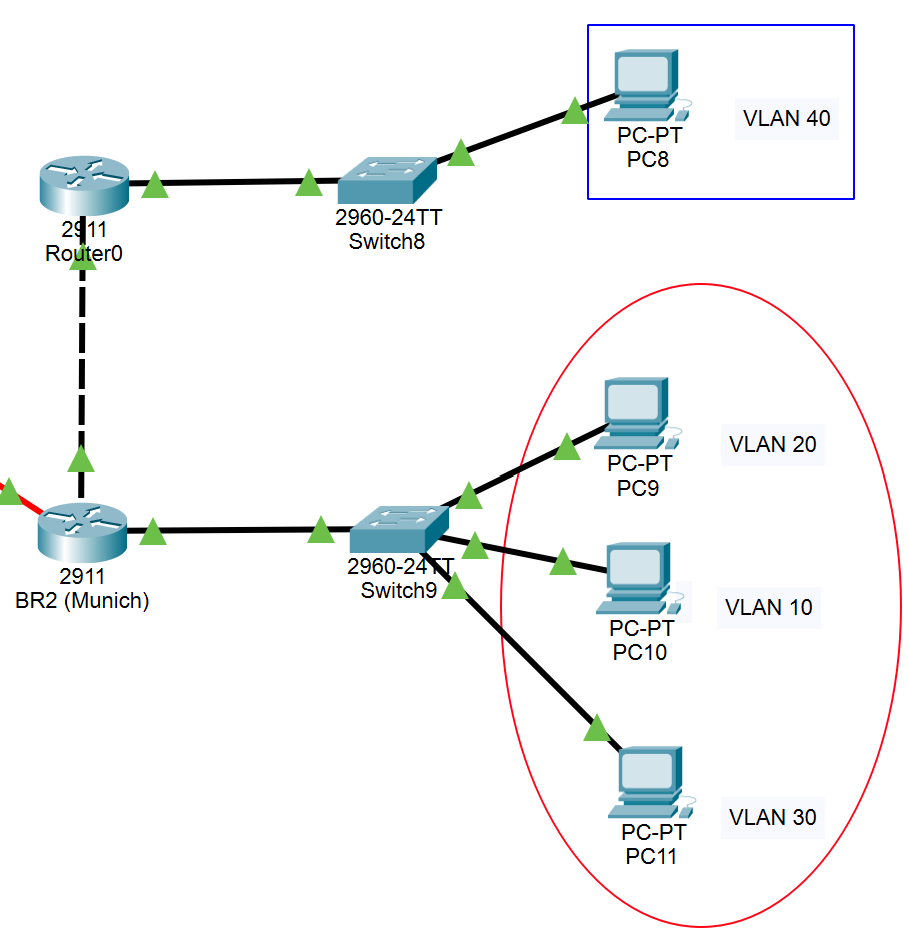
\includegraphics[width=0.6\textwidth]{figures/munich_topology.png}
\caption{\label{fig:munichtopology}Munich WAN Topology}
\end{figure}


\section{Munich Subnet Implementation}

In this subchapter, you will find the addressing for this branch in Table \ref{tab:munich-addressing}. This branch, like the previous one, contains four VLANs, each with a number of nodes, a network address, a broadcast address, a mask, and a range of addresses that can be used for each machine on the network.

\begin{table}[h]
\centering
\resizebox{\textwidth}{!}{%
\begin{tabular}{lccccc}
\hline
\textbf{Network} & \textbf{Number of Nodes} & \textbf{Network Address} & \textbf{Broadcast Address} & \textbf{Mask} & \textbf{First--Last Valid Address} \\
\hline
USERS & 200 & 172.18.78.0 & 172.18.78.255 & /24 & 172.18.78.1 -- 172.18.78.254 \\
ACCOUNTING & 20 & 172.18.79.0 & 172.18.79.31 & /27 & 172.18.79.1 -- 172.18.79.30 \\
STAFF & 10 & 172.18.79.32 & 172.18.79.47 & /28 & 172.18.79.33 -- 172.18.79.46 \\
HR & 10 & 172.18.79.48 & 172.18.79.63 & /28 & 172.18.79.49 -- 172.18.79.62 \\
\hline
\end{tabular}%
}
\caption{Munich \ac{WAN} \ac{IP} addressing scheme}
\label{tab:munich-addressing}
\end{table}


As shown in Figure \ref{fig:munichaddressing}, the addressing for the Munich branch is presented.

\begin{figure}[!htb]
\centering
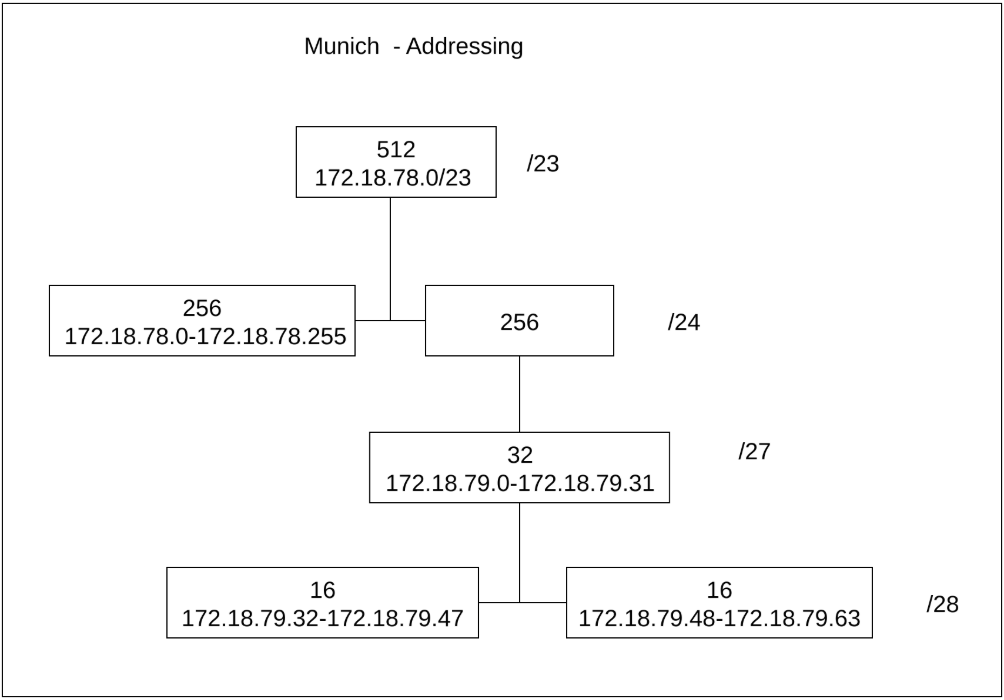
\includegraphics[width=0.6\textwidth]{figures/munich_addressing.png}
\caption{\label{fig:munichaddressing}Munich IP Addressing}
\end{figure}

\section{Implementation of Cisco Commands}

In this Munich branch, the goal was to implement VLAN segmentation, inter-VLAN routing, DHCP address allocation and connectivity between remote sites through static routing.

\subsection*{Switch Configuration}

The Switch7 (SW7), was configured to handle three departments: Staff, Accounting, and Human Resources (HR).
The following VLANs were created:

\begin{lstlisting}[caption={VLAN creation on SW7}, label={lst:sw7-vlan-creation}]
vlan 10
  name STAFF
vlan 20
  name ACCOUNTING
vlan 30
  name HR
vlan 50
  name NATIVE
vlan 99
  name BLACKHOLE
\end{lstlisting}

The trunk link connecting SW7 to router BR2 was configured on the \textit{gigabitEthernet0/1} interface, allowing VLANs 10, 20 and 30 and using VLAN 50 as the native VLAN:

\begin{lstlisting}[caption={Trunk configuration on SW7}, label={lst:sw7-trunk}]
interface gigabitEthernet0/1
    switchport mode trunk
    switchport trunk native vlan 50
    switchport trunk allowed vlan 10,20,30
\end{lstlisting}

The access ports for the end-user PCs were then assigned to their respective VLANs.

\begin{lstlisting}[caption={Access port configuration on SW7}, label={lst:sw7-access}]
interface range fa0/1-5
    switchport mode access
    switchport access vlan 10
    no shutdown
exit

interface range fa0/6-10
    switchport mode access
    switchport access vlan 20
    no shutdown
exit

interface range fa0/11-15
    switchport mode access
    switchport access vlan 30
    no shutdown
exit

interface range fa0/16-24
    switchport mode access
    switchport access vlan 99
    shutdown
\end{lstlisting}

The ports not used were assigned to Blackhole VLAN 99 and administratively shutdown to improve security.

Switch8 (SW8), used for local users in Users VLAN 40, was configured with VLAN 40, 50 and 99:

\begin{lstlisting}[caption={VLAN creation on SW8}, label={lst:sw8-vlan-creation}]
vlan 40
  name USERS
vlan 50
  name NATIVE
vlan 99
  name BLACKHOLE
\end{lstlisting}


Secondly, we configured many different network interfaces for vlan 40 and vlan 99:

\begin{lstlisting}[caption={Access port configuration on SW8}, label={lst:sw8-access}]
interface range fa0/1-24
    switchport mode access
    switchport access vlan 40
    no shutdown
exit

interface range gigabitEthernet0/2
    switchport mode access
    switchport access vlan 99
    shutdown
exit    
\end{lstlisting}

\subsection{Router Configuration}
This subsection demonstrates the configuration of two routers: BR2 and Router0 (R0).
\vspace{0.1cm}
\subsubsection*{BR2}

The BR2 router is connected to the internet with the IP address 193.136.60.147/29. The R0 router is connected to the BR2 router with a crossover cable.

First, the gigabitEthernet0/0 interface was configured, connecting the BR2 router to the internet. Therefore, we have the following code:

\begin{lstlisting}[caption={Interface GigabitEthernet0/0 Configuration}, label={lst:intf-gb0/0}]
interface gigabitEthernet0/0
  ip address 193.136.60.147 255.255.255.248
  no shutdown
exit
\end{lstlisting}

On the BR2 router, four subinterfaces were configured to handle traffic from different VLANs over a single physical interface. Each subinterface is identified by a \texttt{.} followed by the VLAN number, which allows the router to distinguish between the different VLANs. The command \texttt{encapsulation dot1q <VLAN>} specifies that 802.1Q trunking is being used, enabling the physical interface to carry traffic from multiple VLANs simultaneously.

The IP addresses assigned to each subinterface allow the router to act as the default gateway for the hosts in the corresponding VLANs:

\begin{itemize}
    \item GigabitEthernet0/1.10: configured for VLAN 10 with IP address \texttt{172.18.79.46/28}. This subinterface provides routing and inter-VLAN connectivity for devices in VLAN 10.
    \item GigabitEthernet0/1.20: configured for VLAN 20 with IP address \texttt{172.18.79.30/27}, serving as the gateway for devices in VLAN 20.
    \item GigabitEthernet0/1.30: configured for VLAN 30 with IP address \texttt{172.18.79.62/28}, providing routing services for VLAN 30 hosts.
    \item GigabitEthernet0/1.50: configured for VLAN 50 as the native VLAN. No IP address is assigned because this VLAN is likely used only for untagged traffic passing through the trunk, without requiring routing.
\end{itemize}

By assigning unique IP addresses to each subinterface, the router can perform inter-VLAN routing, allowing devices on different VLANs to communicate while still maintaining VLAN segmentation. This setup efficiently leverages a single physical interface to carry multiple networks, reducing hardware requirements and simplifying the network topology.

\begin{lstlisting}[caption={Subinterfaces configuration on BR2 router}, label={lst:subintf-BR2}]
interface gigabitEthernet0/1.10
  encapsulation dot1q 10
  ip address 172.18.79.46 255.255.255.240

interface gigabitEthernet0/1.20
  encapsulation dot1q 20
  ip address 172.18.79.30 255.255.255.224

interface gigabitEthernet0/1.30
  encapsulation dot1q 30
  ip address 172.18.79.62 255.255.255.240

interface gigabitEthernet0/1.50
  encapsulation dot1q 50 native
  no ip address
\end{lstlisting}


Next, using the \textit{no shutdown} command, the interface connecting BR2 to SW7 was enabled.

\begin{lstlisting}[caption={Turn on Interface GigabitEthernet0/1 between SW7 and BR2}, label={lst:sw7-BR2}]
interface gigabitEthernet0/1
  no shutdown
exit
\end{lstlisting}

\vspace{0.1cm}
\subsubsection*{R0}

Router R0 is connected to a switch, and that switch has only one associated VLAN, that's VLAN 40, which is USERS. 
First, the GigabitEthernet0/0 interface was configured to connect router BR2 to router R0 with the IP address 193.136.60.148/29 on R0 side.

\begin{lstlisting}[caption={Interface GigabitEthernet0/0 configuration on R0}, label={lst:r0-br2connection}]
interface gigabitEthernet0/0
  ip address 193.136.60.148 255.255.255.248
  no shutdown
exit
\end{lstlisting}

Next, the interface connecting R0 to SW8 was configured. The IP address assigned in the configuration of this interface was 172.18.78.254/24.
\begin{lstlisting}[caption={Configuring the GigabitEthernet0/1 interface on R0}, label={lst:r0-if_gb0/0}]
interface gigabitEthernet0/1
  ip address 172.18.78.254 255.255.255.0
  no shutdown
exit
\end{lstlisting}


\subsection{DHCP Configuration}
In this subchapter, we will explain the DHCP configuration on the two Munich WAN routers for the VLANs of each of the two switches in this network.
DHCP, basically, is a protocol that automatically assigns IP addresses and other network settings, (for example: gateway, DNS) to devices on a network.

\vspace{0.1cm}
\subsubsection*{BR2 Router}
On the BR2 router, three DHCP pools were configured, corresponding to the VLANs connected to the SW7 switch: VLAN 20 (STAFF), VLAN 10 (ACCOUNTING), and VLAN 30 (HR).  
Each pool defines a specific IP range, the respective default gateway, DNS server, and same domain name to be distributed to the hosts within that VLAN. Additionally, several IP addresses were excluded to prevent them from being assigned dynamically—typically reserved for network devices such as routers and switches.

\begin{lstlisting}[caption={Exclusion of static addresses already defined to avoid errors}, label={lst:errors}]
ip dhcp excluded-address 172.18.79.33 172.18.79.45
ip dhcp excluded-address 172.18.79.1 172.18.79.29
ip dhcp excluded-address 172.18.79.49 172.18.79.61
\end{lstlisting}

\begin{lstlisting}[caption={Creation of a DHCP pool called STAFF}, label={lst:staff-pool}]
ip dhcp pool STAFF
 network 172.18.79.32 255.255.255.240
 default-router 172.18.79.46
 dns-server 8.8.8.8
 domain-name RECOMP2526M1A06.recomp.com 
exit
\end{lstlisting}

\begin{lstlisting}[caption={Creation of a DHCP pool called ACCOUNTING}, label={lst:ACCOUNTING-pool}]
ip dhcp pool ACCOUNTING
 network 172.18.79.0 255.255.255.224
 default-router 172.18.79.30
 dns-server 8.8.8.8
 domain-name RECOMP2526M1A06.recomp.com
exit
\end{lstlisting}

\begin{lstlisting}[caption={Creation of a DHCP pool called HR}, label={lst:HR-pool}]
ip dhcp pool HR
 network 172.18.79.48 255.255.255.240
 default-router 172.18.79.62
 dns-server 8.8.8.8
 domain-name RECOMP2526M1A06.recomp.com
exit
\end{lstlisting}

This configuration ensures that each VLAN has its own DHCP scope, allowing devices in each network to automatically obtain an IP address, gateway, and DNS information corresponding to their VLAN. 


The use of excluded address ranges guarantees that static IPs assigned to infrastructure components will not conflict with dynamically assigned addresses.
It should be noted that this DHCP configuration in Packet Tracer will have significant positive effects on PC9 (Vlan 20), PC10 (Vlan 10) and PC11 (Vlan 30).

\newpage
For example, if you look at the DHCP settings on PC9 in the following figure \ref{fig:munich_pc9}, you will see that it corresponds to Code \ref{lst:staff-pool} and that it contains exactly the assigned DNS IP (Google) and the corresponding default-gateway from the Staff Pool.

\begin{figure}[!h]
\centering
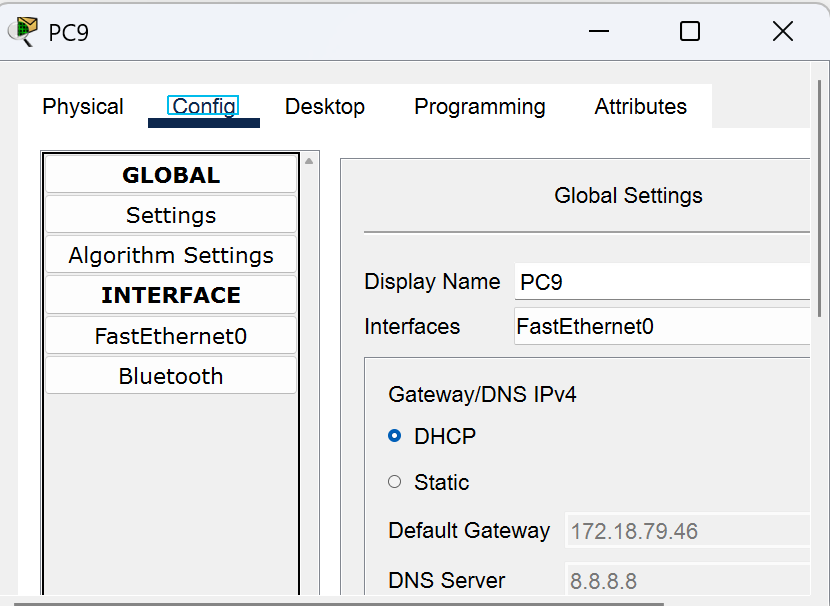
\includegraphics[width=0.5\textwidth]{figures/pc9_conf_example.png}
\caption{\label{fig:munich_pc9}Demonstration of PC9 DNS and your Default-Gateway}
\end{figure}

\subsection{IP Route Configuration}

In this subsection, the configuration of IP routes in packet tracer on router BR2, as well as on router R0, is demonstrated. 
\vspace{0.1cm}
\subsubsection*{BR2}

\begin{lstlisting}[caption={IP Route Demonstration of BR2 Router}, label={lst:br2router_iproute}]
ip route 172.18.78.0 255.255.255.0 193.136.60.148
\end{lstlisting}

In the Code \ref{lst:br2router_iproute}, it can be seen that there is an IP designated by \textit{172.18.78.0} which is the network address of router R0, followed by the network mask /24, and finally there is the IP address \textit{193.136.60.148} which is the IP of the next-hop or the IP of the neighboring router, i.e. is, the IP of Router0 where the traffic will be sent and reach the destination network.

\vspace{0.1cm}
\subsubsection*{R0}
In this subsection, the configuration of static IP routes in Packet Tracer on Router0 is presented. 

\begin{lstlisting}[caption={IP Route Demonstration of Router0}, label={lst:router0_iproute}]
ip route 172.18.79.0 255.255.255.224 193.136.60.147
ip route 172.18.79.32 255.255.255.240 193.136.60.147
ip route 172.18.79.48 255.255.255.240 193.136.60.147
\end{lstlisting}

In the Code \ref{lst:router0_iproute}, it can be observed that three static routes are configured on Router0. The first route defines the network \textit{172.18.79.0/27}, the second route defines the network \textit{172.18.79.32/28}, and the third route defines the network \textit{172.18.79.48/28}. All these networks are reachable through the next-hop IP address \textit{193.136.60.147}, which corresponds to the neighboring router BR2. 

Therefore, these static routes allow Router0 to forward traffic destined for the mentioned networks through BR2, ensuring proper communication between the subnets and the rest of the topology.


\chapter{Conclusion}

The development of RECOMP Corporation's WAN during Sprint 1 represented a crucial milestone in establishing a functional, scalable, and secure network infrastructure, interconnecting the company's three main facilities — Porto (headquarters), Warsaw, and Munich. Throughout this phase, key objectives were successfully achieved, including the design and implementation of IP addressing schemes, the configuration of VLANs and VTP domains, the deployment of redundancy protocols, and the validation of internal and external connectivity.

At the Porto headquarters, the configuration of multilayer switching, VLAN segmentation, and redundancy protocols such as HSRP ensured high availability and resilience against potential network failures. The use of VTP and DHCP services further simplified network management and automation.

In Warsaw, the implementation of a structured subnet plan and the correct configuration of redundancy mechanisms such as HSRP ensured seamless gateway failover and optimised routing performance. The implementation of DHCP pools for each VLAN confirmed proper network segmentation and automated address management.

Similarly, in Munich, routing between VLANs, trunking, and DHCP configuration were successfully implemented, ensuring connectivity between departments and between networks through static routing. The logical separation of VLANs and the configuration of subinterfaces on the routers enabled efficient communication between all networks on different VLANs.
 
This first sprint laid the foundation for RECOMP Corporation's enterprise network. Each site now operates with a consistent addressing scheme and stable connectivity to the Internet and between each machine (e.g., PCs) on each WAN.



Finally, all objectives set for Sprint 1 were fully achieved. RECOMP's WAN is now operational and ready for the next phases of development.


\bibliographystyle{plain} % Choose the style of your references
\bibliography{refs} % Link your .bib file here

\end{document}



